\documentclass[a4paper,12pt]{article}
\usepackage[english]{babel}
\usepackage[utf8]{inputenc}
\usepackage[T1]{fontenc}
\usepackage{indentfirst}
\usepackage[top=2.5cm, bottom=2.5cm, left=2.5cm, right=2.5cm]{geometry}
\usepackage{amsmath}
\usepackage{hyperref}
\usepackage{graphicx}

\graphicspath{ {./img/} }
\title{ML Nanodegree Capstone Project\\Investment and Trading application}
\author{Maciej Nalepa}
\date{2020 January}
\begin{document}
\maketitle

\part{Definition}
\section*{Project Overview}
Knowing the future of a market stock price is a very valuable information about risk of investment and is commonly pursued because of potentially infinite profits.

Currency ratio and stock markets forecasting based on technical analysis can be easily implemented in a script thanks to a timeseries prediction nature of the problem. Price and volume are publicly accessible and can be used to train a model aiming to output the most likely future price.

In this project I have explored different Machine Learning techniques to find the best predictor of stock market values.

Project was inspired by personal experience in development of trading algorithms.

\section*{Problem Statement}
We want to predict the price of EURUSD ratio and NASDAQ stock. It is a timeseries forecasting problem. The goal is to create a model that will forecast future values basing on input provided as a starting point. Then a web application will serve forecasts live by downloading information from third party services.

\section*{Evaluation Metrics}
Because we are developing regression model a norm metric is required. For our purposes we will use Mean Squared Error (MSE) between predicted $y$ and actual values $\hat{y}$ (\ref{MSE}). Model loss is calculated from N predictions against actual values.

Evaluation will be performed on test data which is the 20\% tail of our datasets. Performance will be compared to a simple MA prediction solution (\cite{Vidhya}).
\begin{equation}
	\label{MSE}
	MSE = \frac{1}{2} \left( y - \hat{y} \right)^2
\end{equation}

%%%%%%%%%%%%%%%%%%%%%%%%%

\part{Analysis}
\section{Data Exploration}
Data is represented with "candles". Each candle is stored in one row of our dataset and it is defined with a datetime stamp. Timeframe represents how long is each candle lifespan, 1 minute being the shortest and technically with no upper limit, but usually it is not common to get data with timeframe longer than 1 month.
The dataset I have acquired consists of 5 years NASDAQ stock market history with 1-day timeframe (source: Yahoo! Finance \cite{Yahoo}). Another dataset is 5 years of EURUSD history with 1-minute timeframe (source: HistData \cite{HistData}).

Market data consists of four basic columns: Open, High, Low, Close and for stock markets: Volume.

\begin{itemize}
	\item Open -- the price value when a candle was initiated.
	\item High -- highest price reached during candle lifespan.
	\item Low -- lowest price reached.
	\item Close -- the price at which the candle lifespan passed.
	\item Volume -- the number of shares that changed during candle lifespan.
\end{itemize}

There are important differences between NASDAQ and EURUSD data. First currency pairs do not have Volume, so this data is missing and for convenience I will drop this column from NASDAQ as well. Another aspect is the value difference, NASDAQ ranges from $4000$ to $9000$, while EURUSD was much more stable for last 5 years staying around $1.15$. EURUSD will be converted to 1-day timeframe, so it matches the other dataset. Such change greatly reduces the amount of entries, which makes working with this data faster (for the cost of information loss).

\begin{figure}[h]
	\centering
	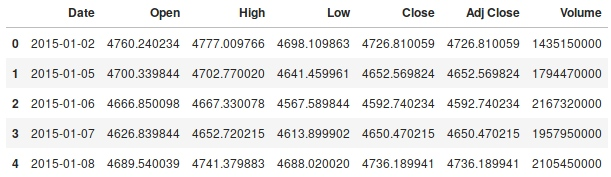
\includegraphics[width=\textwidth]{nasdaqTable}
	\caption{Sample of market data (NASDAQ)}
\end{figure}

\section{Visualization}
It is vital to have the values correctly distributed. Market is unbalanced and the prices can range from 0 to infinity. For training it is best when the dataset has normal distribution (\cite{Distribution}), the histograms below do show that some kind of normalization will be needed.
EURUSD overall looks closer to what we need, but it is possible to get it better than that using normalization techniques.

Market data actually is normally distributed but only on short samples and only if there is no strong trend in the sample (in such case distribution looks more like NASDAQ histograms).

\begin{figure}[h]
	\centering
	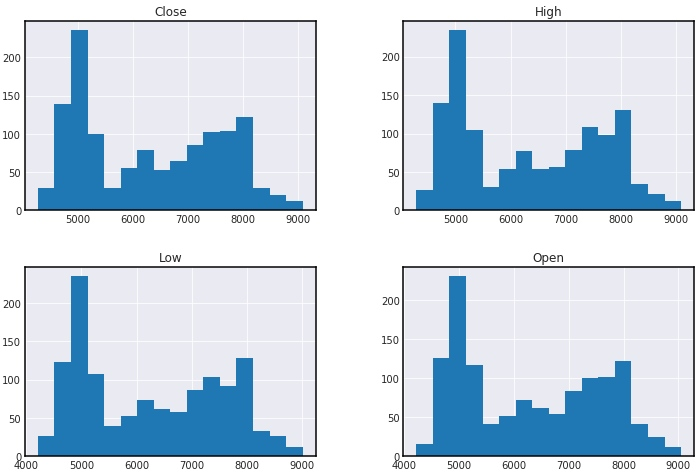
\includegraphics[scale=2.2]{nasdaqHist}
	\caption{Histograms (NASDAQ)}
\end{figure}
\begin{figure}[h]
	\centering
	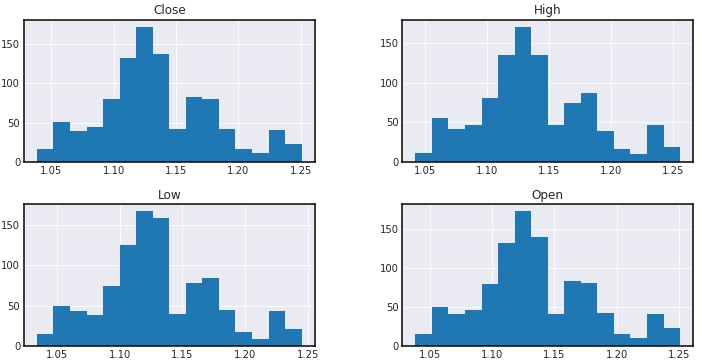
\includegraphics[scale=2.2]{eurusdHist}
	\caption{Histograms (EURUSD)}
\end{figure}

\section{Algorithms \& Techniques}
The regressor uses Long Short Term Memory, which is one of the best currently known methods for working with timeseries data and any other position dependent information sets (e.g. words in a sentence). This model is based on PyTorch framework (\cite{Torch}).

Architecture of the model is 1-D Batch Normalization over the input split into channels, which are the columns of our data making predictor independent of the input scale. Then 1-D Convolution is applied, which allows to extract more information from the input. Combination of these methods allow the model to work with both datasets in the state as they are -- no scaling is required during data preprocessing.

Normalized input is flattened finally passed to fully connected layer, which outputs predictions for $N$ future Close price values. Output is in normalized space though and a function to denormalize output into correct value is required (\ref{denorm}).
\begin{equation}
\label{denorm}
prediction = std(input[Close]) * output + input[Close].last
\end{equation}

Web application is an HTML document using javascript to retrieve forecasts on demand. User provides any Yahoo symbol as a string and receives forecast for it as a json response. Received data is plotted using Plotly \cite{Plotly}.

\section{Benchmark Model}
The only way to tell how good the model will perform is to compare it with another solution. Moving Average prediction is a great option here. It assumes that next value is the average of last $N$ observations, where $N$ is the count of observed values. It turned out that the value of $N = 2$ is the best. There is a good visualization of how this works \cite{Vidhya}.
\begin{figure}[h]
	\centering
	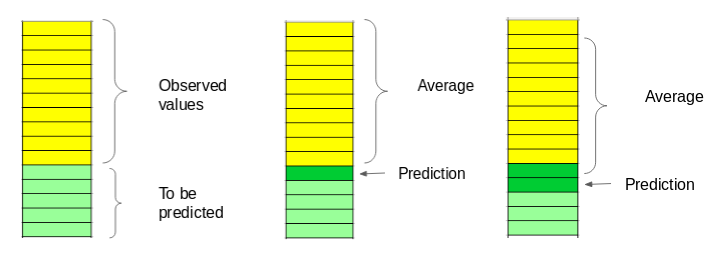
\includegraphics[scale=0.5]{ma}
	\caption{Moving Average prediction sequence \cite{Vidhya}}
\end{figure}

%%%%%%%%%%%%%%%%%%%%%%%%%

\part{Methodology}
\section{Data Preprocessing}
As stated in the Algorithms \& Techniques section there is no need to scale the data, predictor will do it on its own.
Instead of modifying the data it is possible to calculate some indicators knowing only the previous Open, High, Low and Close prices. This way we can generate some new features:
\begin{itemize}
	\item Gap -- days between entries, market is shut down for holidays resulting in gaps in the data.
	\item EMA -- exponential moving average.
	\item SMA -- simple moving average.
	\item Momentum -- value change indicator.
	\item RSI -- relative strength index oscillator.
\end{itemize}

\begin{figure}[h]
	\centering
	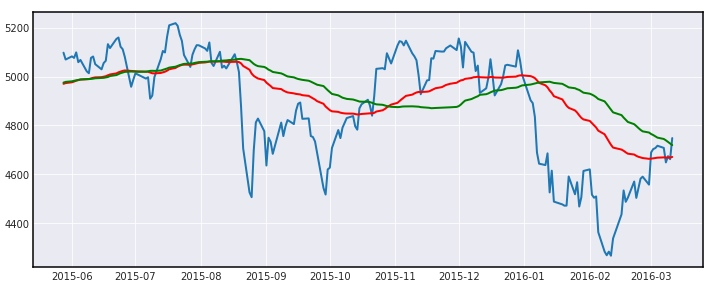
\includegraphics[height=6cm,width=\textwidth]{nasdaqClose}
	\caption{(NASDAQ) Close price (blue) with EMA (red) and SMA (green) indicators}
\end{figure}
\begin{figure}[h]
	\centering
	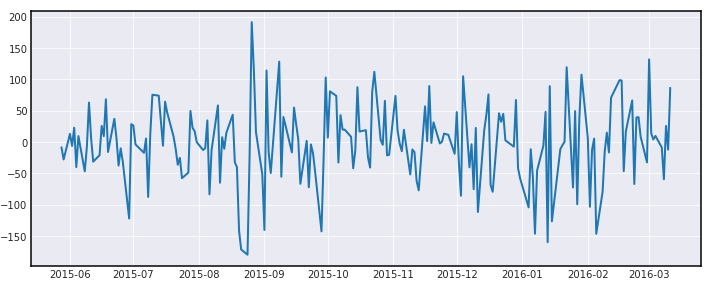
\includegraphics[height=4cm,width=\textwidth]{nasdaqMom}
	\caption{(NASDAQ) Momentum}
\end{figure}
\begin{figure}[h]
	\centering
	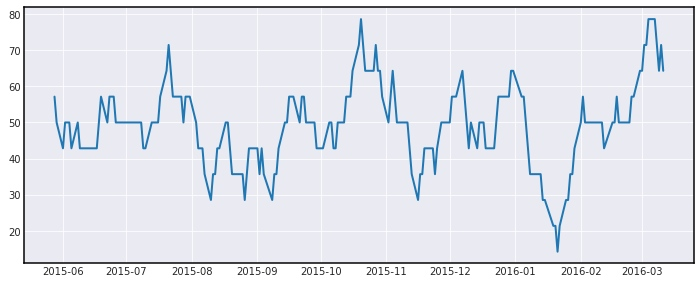
\includegraphics[height=4cm,width=\textwidth]{nasdaqRSI}
	\caption{(NASDAQ) Relative Strength Index}
\end{figure}

\section{Implementation}
The easiest way to describe implementation steps is to follow the notebooks and specify which scripts they use and what do they do.

In the \texttt{Analysis} notebook \texttt{utils.py} was imported. It contains definitions for loading the data from \texttt{.csv} files and changing data timeframe. To apply some basic indicators a separate module was created for the needs of this project. The module has definitions for indicators SMA, EMA, Momentum and RSI oscillator (\cite{Indicies}). These are enough to get working with the \texttt{Analysis} notebook and export datasets into csv train and test files.

The next 2 notebooks are using the \texttt{model} directory which is the source dir for both training and deployment. There is \texttt{model.py} which contains definitions for LSTMRegressor, SlidingWindowDataset, denormalization function and model\textunderscore fn. Another files are the required modules and scripts used for training or prediction once deployed.

Next \texttt{Model} notebook works with \texttt{model.py} and \texttt{train.py} files from the \texttt{model} directory which is used as a source dir for deployment. This notebook creates benchmark MA model, optimizes it, tests input and training of LSTM model, starts SageMaker training with specified parameters and finally compares predictions losses of the 2 methods directly.

The last notebook is the \texttt{WebApp} which basically takes care of getting the correct files into the source dir, tests yfinance module and deploys the RealTimePredictor, so we can use it from the web application.
The Webapp is just one HTML file that uses javascript to send requests to the Lambda through API Gateway, there are a lot of steps to get it running on AWS but the HTML itself requires only setting the API url. I wanted to make this more interesting by allowing the webapp to run predictions on any symbol live using a nice Python module for collecting data from Yahoo! \cite{yf}.

\section{Refinement}
Currently, the predictor is fixed to use the output size as the horizon of predictions. This means that output size of $N$ will make the model train to predict $N$ future values. This is just implementation because in this project there were no models trained with output size larger than 1.

%%%%%%%%%%%%%%%%%%%%%%%%%

\part{Results}
\section{Model Evaluation and Validation}
After 100 epochs on NASDAQ the loss reached 35382 (train) / 850213 (test), but it was greatly overfitted, because since epoch 30 the test loss was increasing.

EURUSD looked similarly, after 30 epochs started overfitting. Final loss was 0.000365 (train) / 0.001459 (test).

\begin{figure}[h]
	\centering
	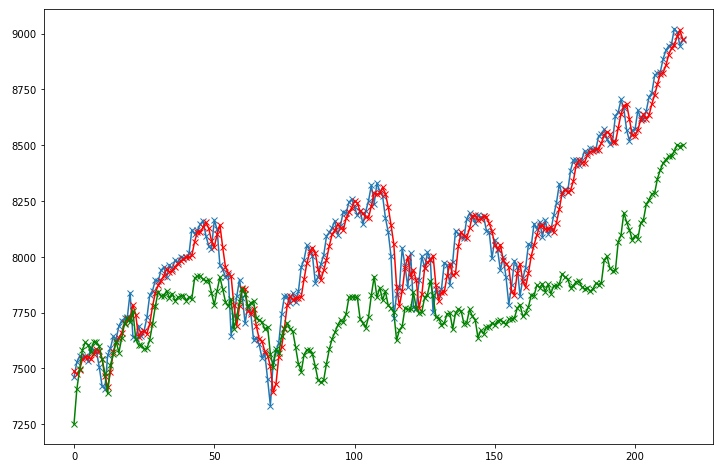
\includegraphics[scale=2.2]{nasdaqVs}
	\caption{Blue: actual close, red: MA prediction, green: LSTM predicition. Error for NASDAQ was almost 18x the error of benchmark.}
\end{figure}

\begin{figure}[h]
	\centering
	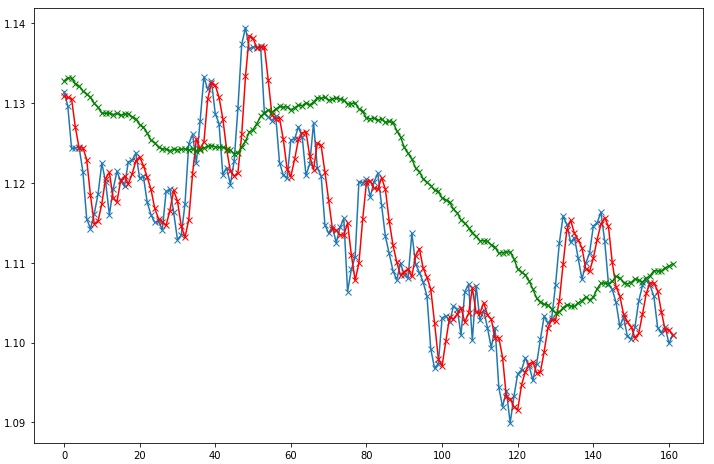
\includegraphics[scale=2.2]{eurusdVs}
	\caption{Blue: actual close, red: MA prediction, green: LSTM predicition. Error for EURUSD was around 8x the error of benchmark.}
\end{figure}

\section{Justification}
Hello

%%%%%%%%%%%%%%%%%%%%%%%%%

\part{Conclusion}
\section{Reflection}
I guess that efficient-market hypothesis has beaten me once again. That is the biggest challenge of this project, forecasting future market price is not an easy task and can cause headaches.

During development of this project I have run into many problems according the predictor architecture. I could not decide on the best way to deconvolve / denormalize the single value output, solution described above (\ref{denorm}) proved to work with best accuracy. I wanted to avoid scaling the dataset for all costs, because that is a common approach and instead allow the model to do the normalizing over input itself.

\section{Further Improvements}
Here the same model was trained on both datasets, which did not prove to provide any better accuracy in forecasting.
It may be better to train separate model for each symbol.

In this work the datasets had combined length of 2250. More data should improve the model.

Predicting High and Low instead may greatly improve usefulness of the forecasts. It is very difficult to accurately predict a price, but a range can be predicted with a higher certainty.

If the model had accuracy above a certain level it may be profitable in a trading or investing strategy once implemented.

%%%%%%%%%%%%%%%%%%%%%%%%%

\pagebreak
\begin{thebibliography}{15}
	
\bibitem{Vidhya}
Aishwarya Singh, \textit{Stock Prices Prediction Using ML and DL Techniques},
\texttt{\href{https://www.analyticsvidhya.com/blog/2018/10/predicting-stock-price-machine-learningnd-deep-learning-techniques-python/}{analyticsvidhya.com}}

\bibitem{TowardsData}
Yibin Ng, \textit{Machine Learning Techniques applied to Stock Price Prediction}, \texttt{\href{https://towardsdatascience.com/machine-learning-techniques-applied-to-stock-price-prediction-6c1994da8001}{towardsdatascience.com}}

\bibitem{Distribution}
Rohit Sharma, \textit{Gaussian distribution}, \texttt{\href{https://medium.com/ai-techsystems/gaussian-distribution-why-is-it-important-in-data-science-and-machine-learning-9adbe0e5f8ac}{medium.com}}

%\bibitem{Khan}
%\texttt{\href{https://www.khanacademy.org/economics-finance-domain/core-finance/stock-and-bonds}{khanacademy.com}}

\bibitem{yf}
Ran Aroussi, \textit{yfinance}, \texttt{\href{https://github.com/ranaroussi/yfinance}{github.com}}

\bibitem{Indicies}
Indicators definitions
\texttt{\href{https://www.fxcm.com/uk/insights/learn-forex-oscillators-and-momentum-indicators/}{fxcm.com}}

\bibitem{Yahoo}
Yahoo! Finance
\texttt{\href{https://finance.yahoo.com}{finance.yahoo.com}}

\bibitem{HistData}
HistData
\texttt{\href{http://histdata.com}{histdata.com}}

\bibitem{Torch}
PyTorch
\texttt{\href{https://pytorch.org/}{pytorch.org}}

\bibitem{Plotly}
Plotly
\texttt{\href{https://plot.ly/javascript/}{plot.ly}}

\end{thebibliography}

\end{document}


























